\section{対話システムの構築}
\label{対話システムの構築}
%\subsection{対話システムの全体像}
本章では,対話システムの構築方法について述べる.対話システムは,ロボットのハードウェアを制御するロボット管理と対話の制御を行う対話管理に分けることができる.対話システムの全体像を図\ref{overview_system}に示す.ロボット管理と対話管理の通信は全てTCPで行う.ロボット管理の各モジュールではそれぞれの部位に対応するロボットの制御を行う.\ref{対話システムを構成するモジュール}節で各モジュールの詳しい説明を行う.対話管理ではユーザの発話を理解し,システムの発話や行為を決定する.\ref{対話管理}節で対話管理について詳しく述べる.

\begin{figure}[th]
    \centering
    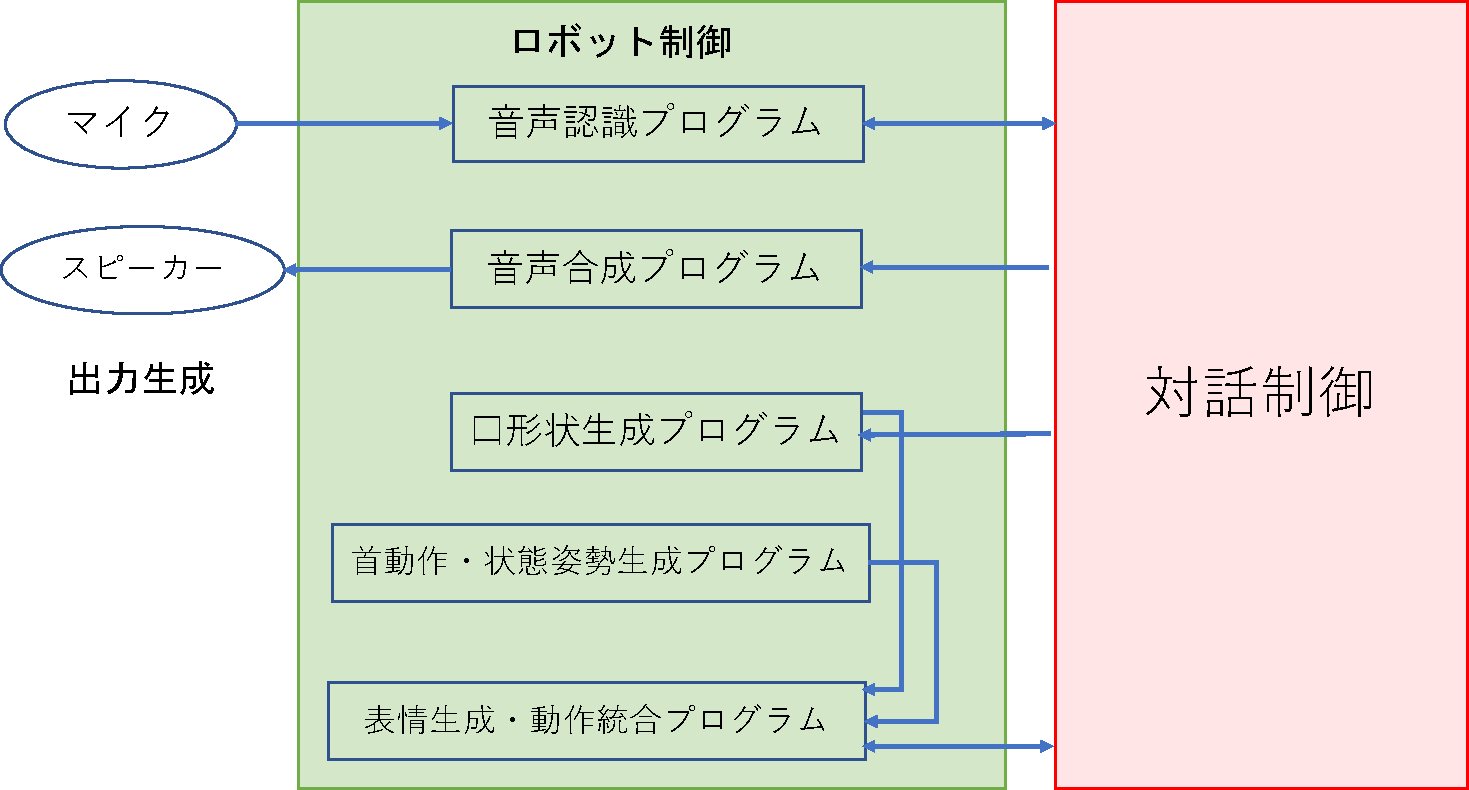
\includegraphics[scale=0.5]{pic/overview_system.pdf}
    \caption{対話システムの全体像}
    \label{overview_system}
\end{figure}

\subsection{ロボット管理}
\label{対話システムを構成するモジュール}
対話ロボットとして,国際電気通信基礎技術研究所(ATR)\footnote{https://www.atr.jp/}が管理するアンドロイドを使用する.身長165センチ,体重38キログラムであり,空気圧アクチュエータで駆動する.本節でロボットを制御するモジュールを詳しく述べる.
\begin{figure}[th]
    \centering
    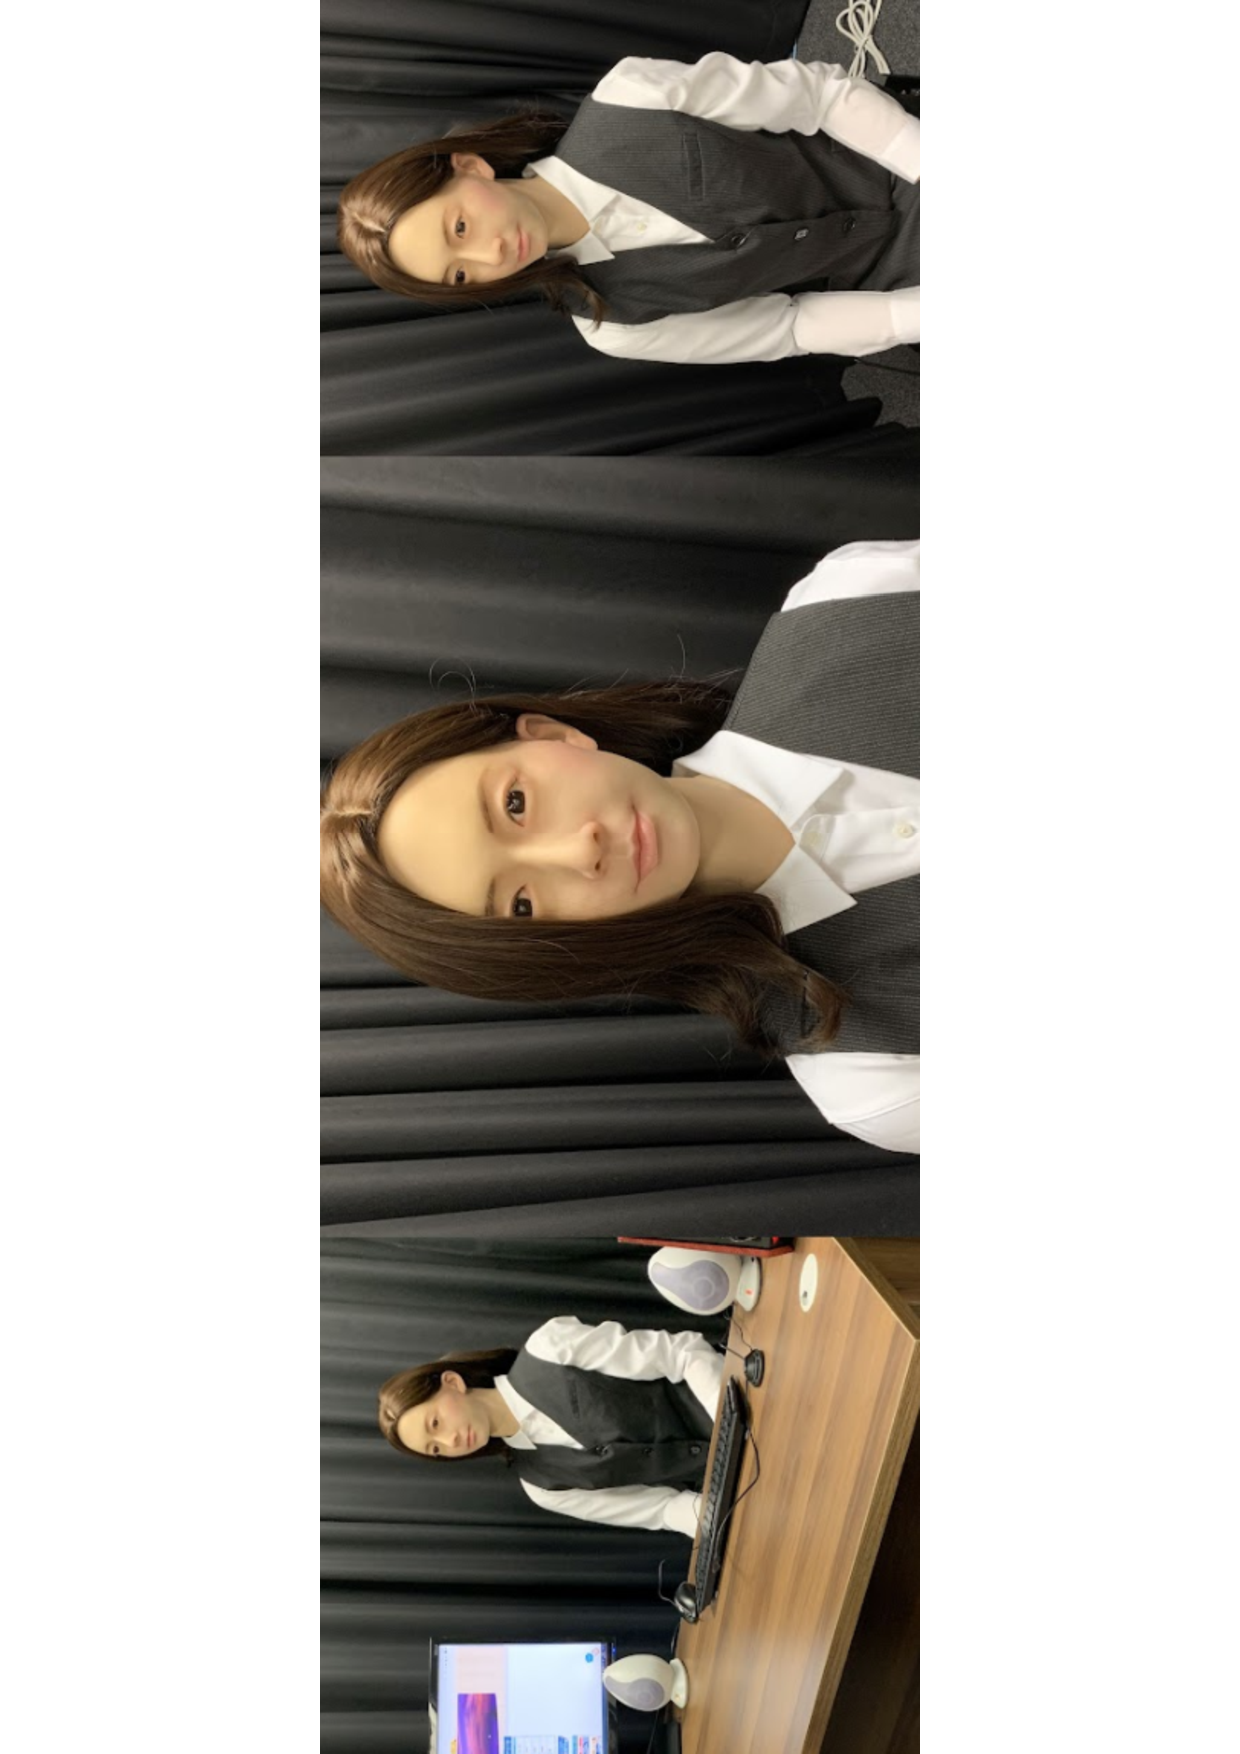
\includegraphics[scale=0.5,angle=270]{pic/ai.pdf}
    \caption{アンドロイドの近景}
    \label{kinkei}
\end{figure}

\subsubsection{音声認識}
音声認識にはGoogleのSpeech-to-Textを利用する.文字コードはutf-8で,音声認識を開始してからマイク入力があると,途中結果を返しながら最終結果と信頼度を返すストリーミング形式の通信を行う.コマンドのフッターは改行コードである.送信プロトコル,受信プロトコルを表\ref{sendrecv}に示す.

\begin{table}[hbtp]
    \caption{送受信プロトコル}
    \label{sendrecv}
    \centering
    \begin{tabular}{l|l}
    \hline
    送信プロトコル                         & 受信プロトコル                  \\ \hline
    音声認識スタート start\textbackslash{}n & 音声認識スタート startrecog:      \\
    音声認識ストップ stop\textbackslash{}n  & 音声認識途中結果 interimresult:  \\
                                    & 音声認識最終結果 result:          \\ 
                                    &  最終結果の信頼度 confidence:       \\ \hline
    \end{tabular}
\end{table}

1度音声認識を開始すると音声認識を終了するまでずっと音声認識をする.受信サンプルを時系列順に並べると以下のようになる.
\begin{table}[hbtp]
    \centering
    \begin{tabular}{|l|}
    \hline
    startrecog:\\
    interimresult:今日\\
    interimresult:今日は\\
    interimresult:今日は\\
    interimresult:今日は週\\
    interimresult:今日は中止\\
    interimresult:今日は中止度\\
    interimresult:今日は修士論文\\
    nterimresult:今日は修士論文発\\
    interimresult:今日は修士論文発表\\
    interimresult:今日は修士論文発表会です\\
    result:今日は修士論文発表会です\\
    confidence:0.9313719153404236\\
    \hline
    \end{tabular}
\end{table}

\subsubsection{音声合成}
音声合成にはAmazonのAmazon Pollyを使用した.通信方式は同期通信で,全てJSON形式でやりとりが行われる.文字コードはutf-8で,コマンドのフッターは改行コードである.再生に成功した場合,
\begin{table}[hbtp]
    \centering
    \begin{tabular}{l}
    \{(送信)再生コマンド $\rightarrow$\\ 
    (受信) \{"result":"success-start","duration":12491\} \\
    $\rightarrow$ (受信)\{"result":"success-end"\}\\
    \end{tabular}
\end{table}    
のように,音声の再生開始,終了と音声の再生時間を受信する.失敗した場合は,
\begin{table}[hbtp]
    \centering
    \begin{tabular}{l}
    \{(送信)再生コマンド $\rightarrow$ (受信)\{"result":"failed"\}
    \end{tabular}
\end{table}
となる.また,

\begin{table}[hbtp]
    \centering
    \begin{tabular}{l}
        (送信)\{"engine":"ISSPEAKING"\} $\rightarrow$(受信)\{"isSpeaking":true/false\}
    \end{tabular}
\end{table}

で現在発話中かを確認することができ,

\begin{table}[hbtp]
    \centering
    \begin{tabular}{l}
        (送信)\{"engine":"STOP"\} $\rightarrow$ (受信)\{"result":"success-end"\}
    \end{tabular}
\end{table}

で再生中に音声を停止することができる.
音声合成に使用するパラメータを表に示す.


システムに標準のピッチ,声量,大きさで「コマンドサンプル」と発話させるためのコマンドの例を以下に示す.
\begin{table}[hbtp]
    \centering
    \begin{tabular}{c}
        \{"engine":"POLLY", "speaker": "Mizuki",  "pitch": 100, "volume":100, \\
        "speed":100,"vocal-tract-length":0, "duration-information":false,  \\
        "speechmark":false, "text":"コマンドサンプル"\}\textbackslash{}n
    \end{tabular}
\end{table}


\subsubsection{口形状生成}
口形状生成には,OculusのOculus Lipsync Unityを利用する.Oculus Lipsync Unityはマイク入力やオーディオファイルからのオーディオインプットストリームを分析し,口形素と呼ばれる唇や顔の表情の一連の値を予測するソフトウェアである.プログラムにアクセスする必要はなく,合成音声を再生すると,それに同期するようにアンドロイドの口形状を制御する.

\subsubsection{首動作・状態姿勢生成}
%MiracleHuman
首動作・状態姿勢生成は非同期通信で行い,コマンドのフッターは改行コード,文字コードはutf-8である.視線,上体姿勢,感情状態を任意の タイミングで指令することができる.ロボットの正面方向をz軸,右をx軸,上をy軸,ロボットの腰の下を原点とした座標系で,x,y,zで視線,顔,体を向ける座標をメートル単位で指定することができる.ロボットの視線を,正面の1.5メートル先,高さ1.2メートルの位置に向ける際のコマンドを以下に示す."translateSpeed"で表される移動速度の単位はメートル毎秒である.
\begin{table}[hbtp]
    \centering
    \begin{tabular}{l}
        EyeController=\{"id": "EyeController","motionTowardObject": "",\\
        "targetMotionMode": 2,"targetPoint": \{"x": 0.0,"y": 1.2,"z": 1.5\},\\
        "translateSpeed": 2.0\}\textbackslash{}n
    \end{tabular}
\end{table}
また,座標指定で動作をせず,事前に定義されたジェスチャを指示することもできる.定義されたジェスチャでは両手の指の開閉や,頭のみ,首のみ,全身を使ったお辞儀,首や視線の縦振り,横振りを指示することができる.

\subsubsection{表情生成・動作統合}
%JointMapperPlusUltraSuperFace
表情生成・対話生成は非同期通信で行い,コマンドのフッターは改行コード,文字コードはutf-8である.事前に定義された表情のラベルにより,頬,口角,眉毛などの位置を制御し,表情を変化させる.表情のラベルを図\ref{labels}に示す.瞬きは支持する必要がなく,定感覚で自動で行われる.

\begin{table}[hbtp]
    \caption{定義された表情ラベル}
    \label{labels}
    \centering
    \begin{tabular}{l|l}
    \hline
    表情名           & 説明              \\ \hline
    MoodBasedFACE   & 基本の表情           \\
    fullsumile      & 笑ったような表情        \\
    angry           & 怒ったような表情        \\
    bad             & 印象の良くない表情       \\
    mouth-a/i/u/e/o & それぞれの母音を発する時の表情 \\ \hline
    \end{tabular}
\end{table}

\subsection{対話管理}
\label{対話管理}
対話管理では,音声認識した発話を文字列で受け取り,発話理解をし,対話のフローとフレーム表現を含めた内部状態の更新,参照を繰り返しながら行動選択,発話生成を行う.本研究で構築する対話システムは「旅行先の決定」というゴールを持ったタスク指向型対話システムである.対話管理で構成する対話の全体の流れを図\ref{flow}に示し,本システムの想定する対話の流れを詳しく述べる.

\begin{figure}[th]
    \centering
    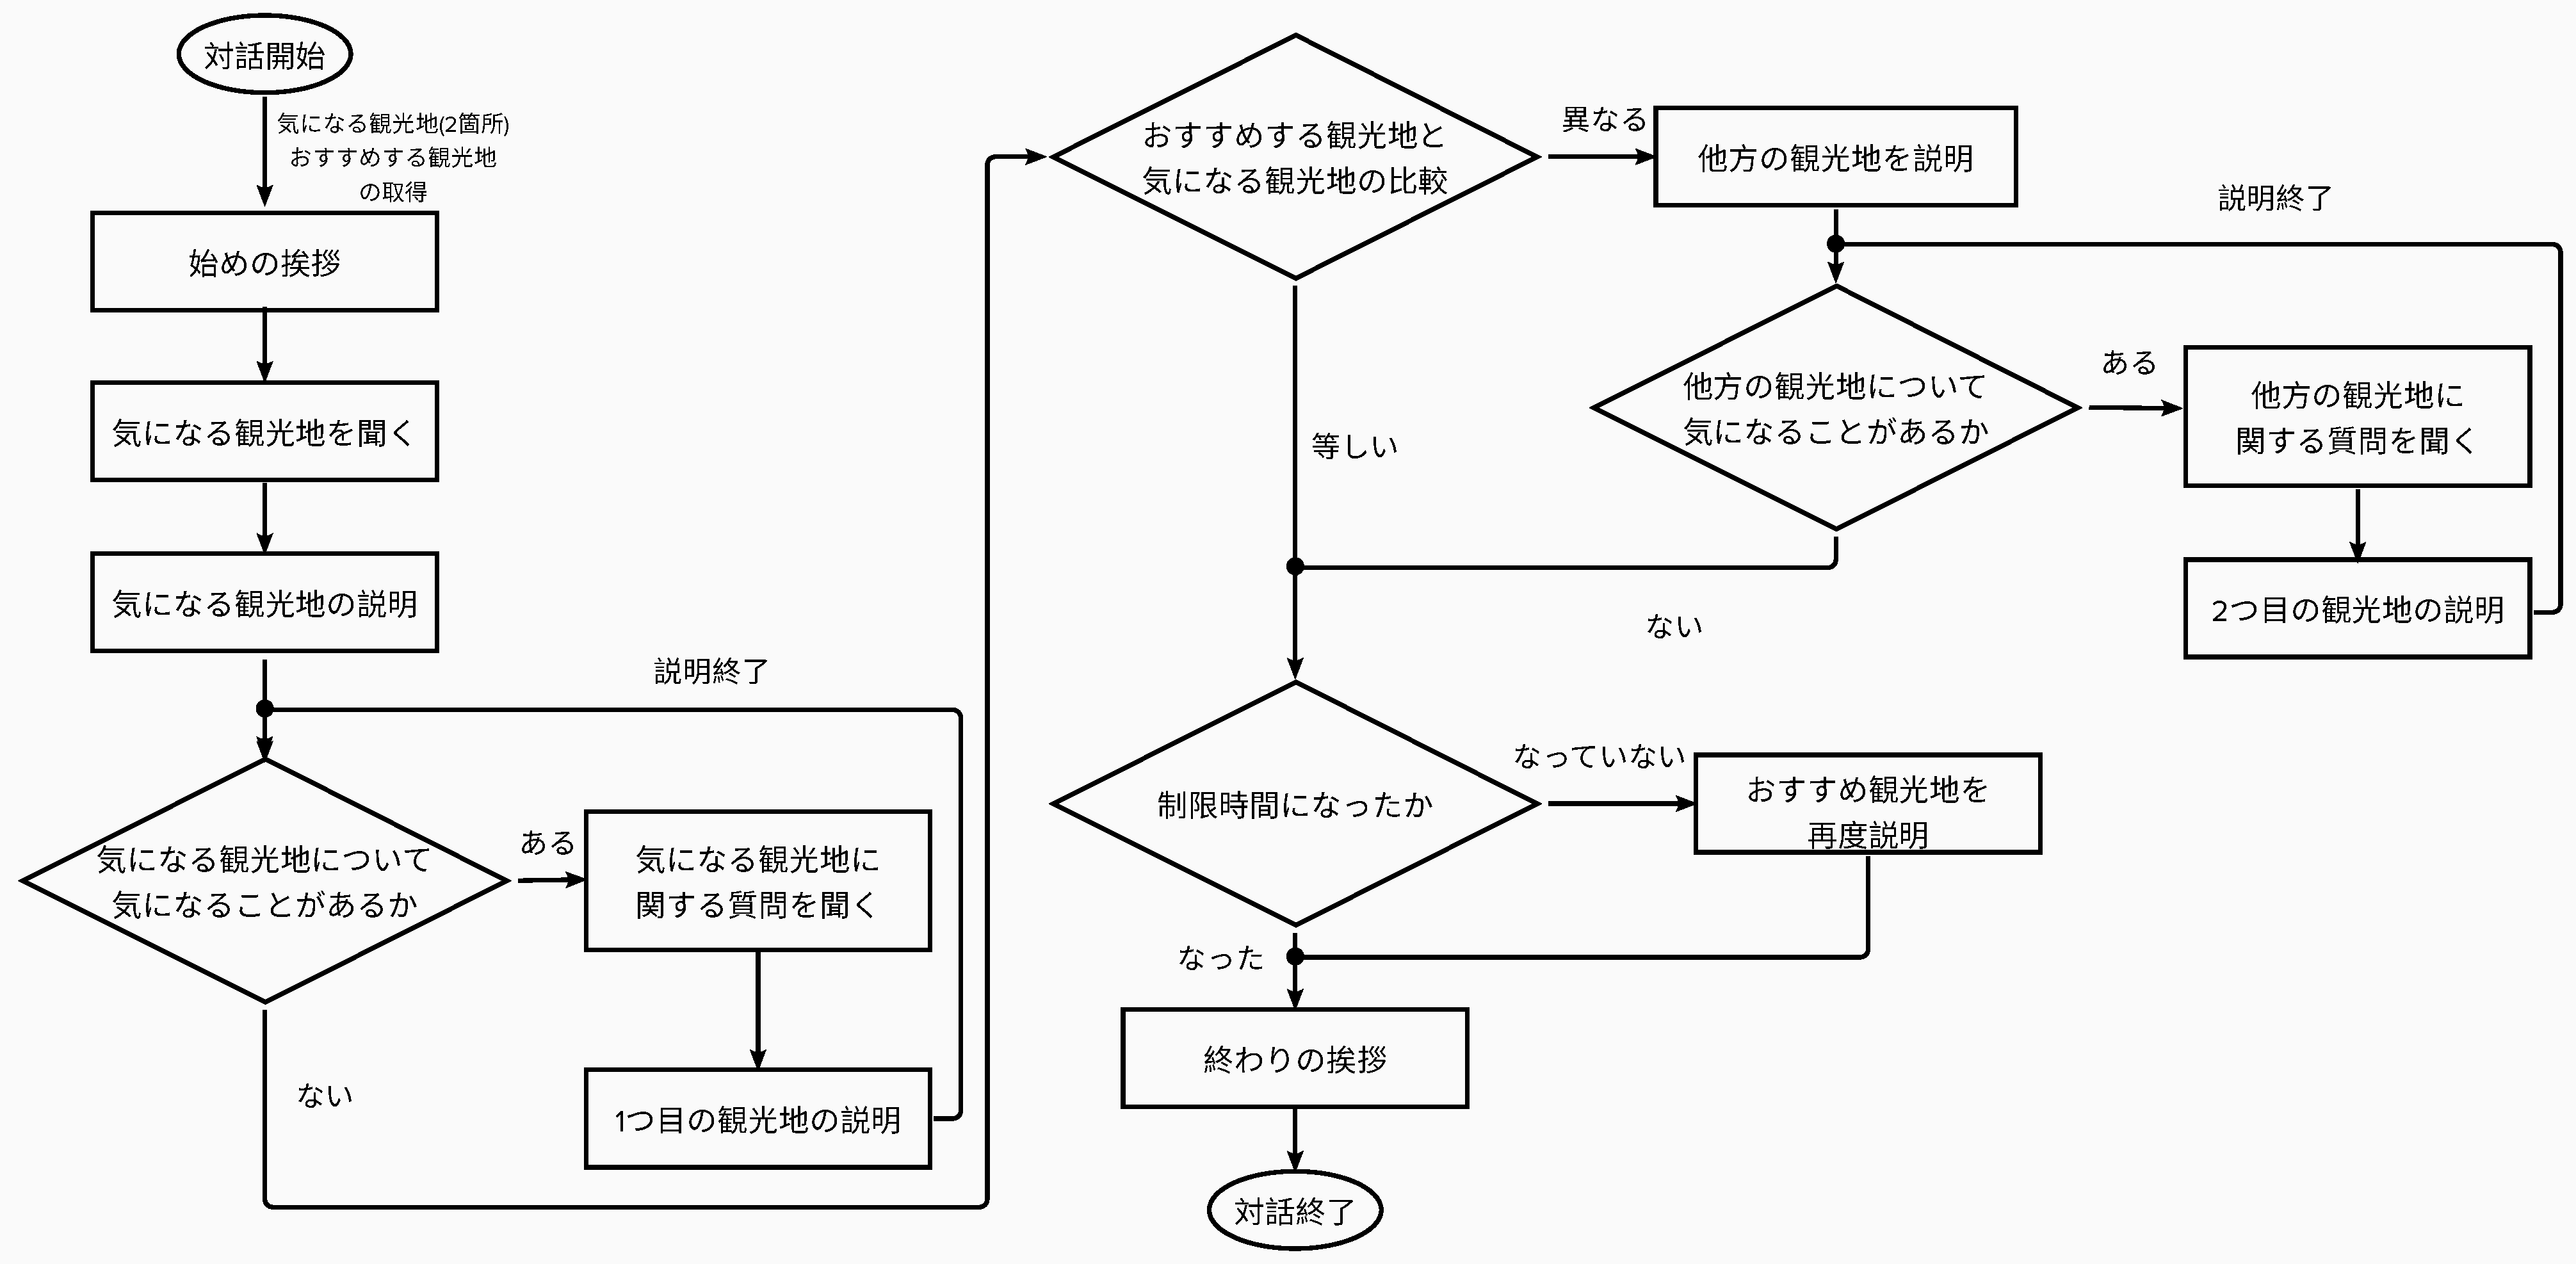
\includegraphics[scale=0.18]{pic/flow.pdf}
    \caption{対話の流れ}
    \label{flow}
\end{figure}

\begin{enumerate}
    \item 対話開始\\
            対話を開始すると,事前にID管理サーバへアクセスし,対話者の選択した2つの観光地と,おすすめ観光地(体験者に選ばせればコンペティションの評価の上がる運営がランダムに選定した勧めるべき観光地.)を取得する.選択した観光地についてどちらの観光地が気になるかを尋ね,気になる観光地の基本情報を説明する.
            \begin{figure}[th]
                \centering
                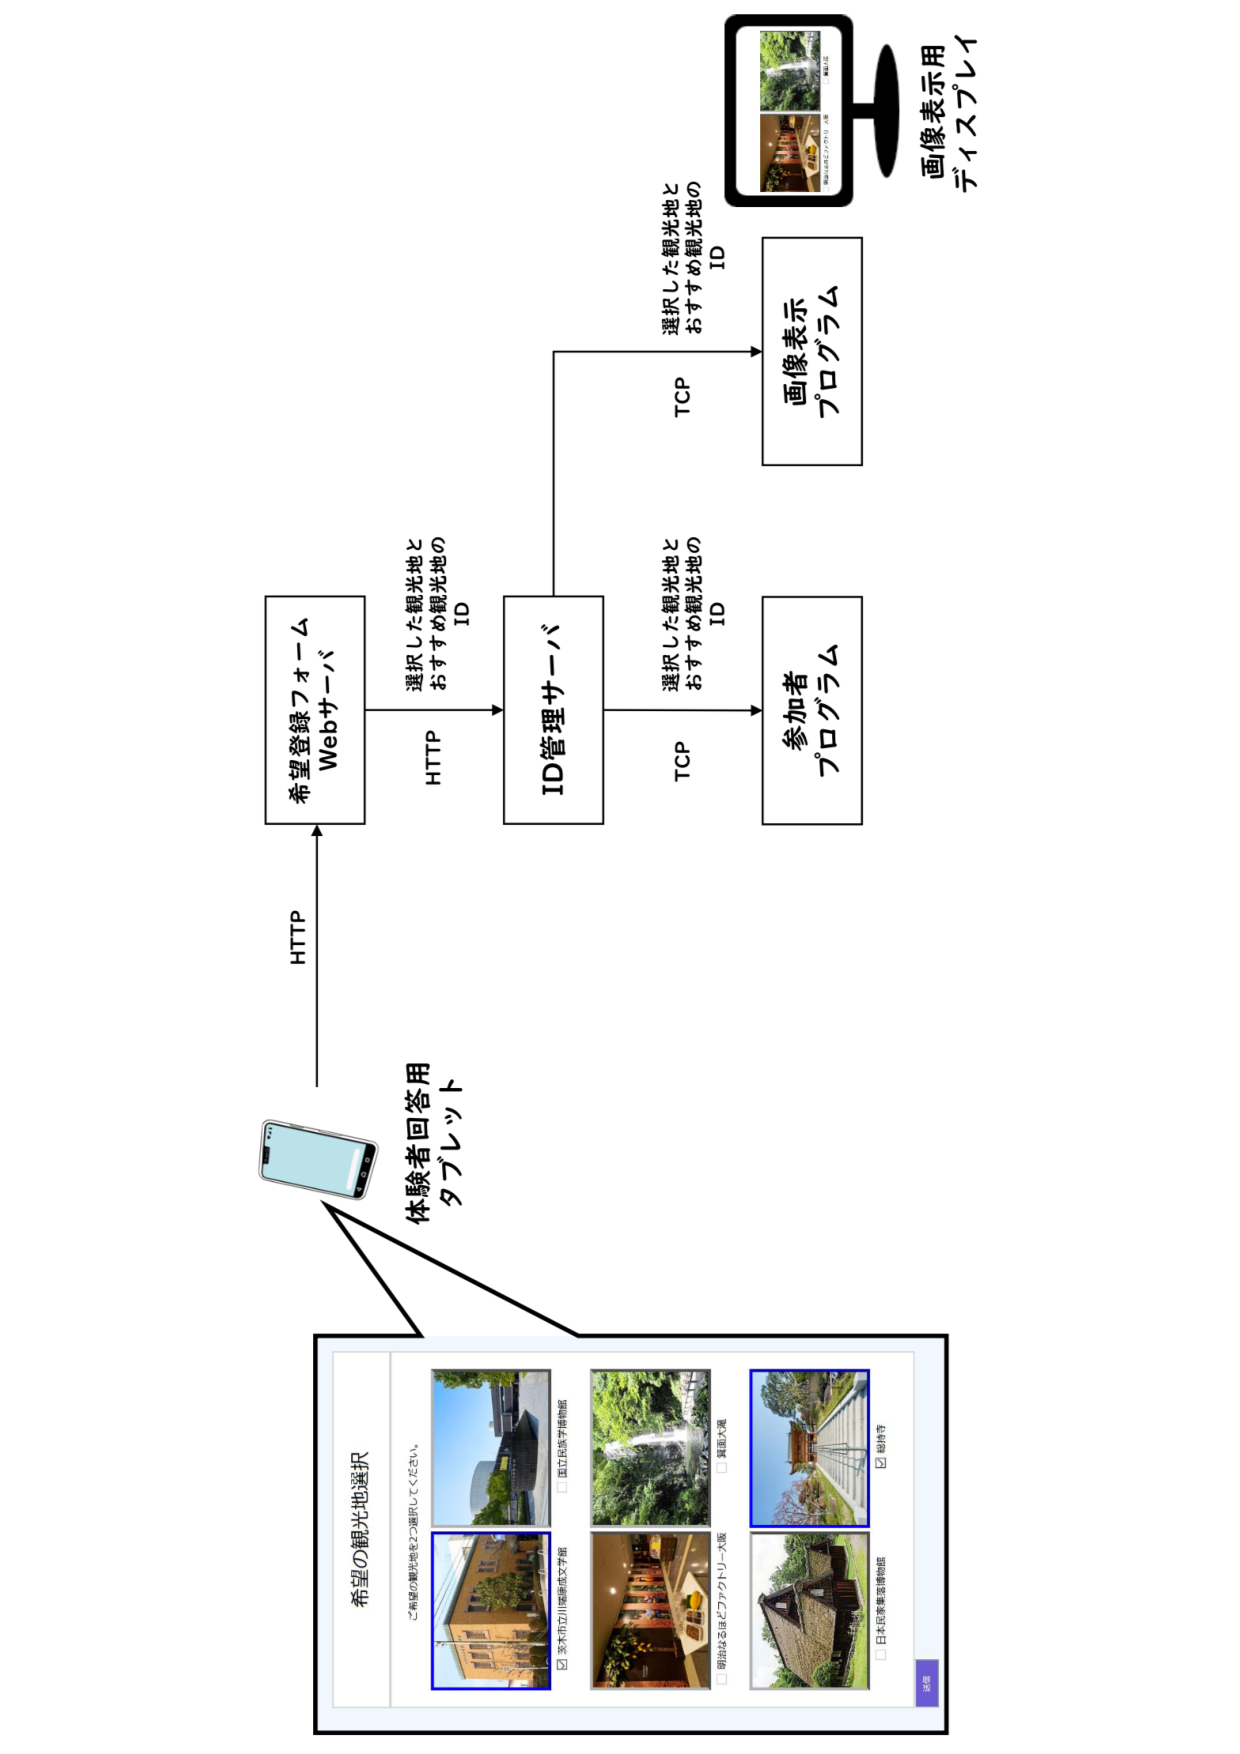
\includegraphics[scale=0.4,angle=270]{pic/how2choice.pdf}
                \caption{観光地の選択システム}
            \end{figure}

    \item 気になる観光地に関する質疑応答\\
            基本情報の説明ののち,「観光地に関して何か気になることはないか」と尋ね,質問がなくなるまで対話者主導で複数回の質疑応答を行う.

    \item 気になる観光地とおすすめ観光地の比較\\
            質問がない場合,気になる観光地とおすすめ観光地の比較を行う.気になる観光地とおすすめ観光地が等しい場合,他方の観光地の説明は行わず,再度気になる観光地についての簡単な説明を行い対話を終了する.気になる観光地とおすすめ観光地が異なる場合は他方の観光地の基本情報を追加で説明する.

    \item 他方の観光地に関する質疑応答\\
            基本情報の説明ののち,「観光地に関して何か気になることはないか」と尋ね,質問がなくなるまで対話者主導で複数回の質疑応答を行う.

    \item 対話終了\\
            他方の観光地について質問が無くなった場合,対話の終了フェーズに入る.定められた対話時間がまだ残っている場合,再度気になる観光地についての簡単な説明を行い対話を終了する.対話時間が来た際は質疑応答の途中でも終わりの挨拶をして対話を終了する.
 \end{enumerate}

 \subsection{言語理解}
 言語理解では対話者の発言から対話行為を推定する.推定には単純な文字列マッチングを用いる.MeCabを用いた形態素解析を行い,ユーザの発言と対話行為タイプの一致判定により対話行為タイプを決める.

\subsubsection{フレーム表現を用いた発話理解}
本システムは「フレーム」と呼ばれるデータ構造を用いて対話を進める.図\ref{frame}に示すように,対話者が事前に選択した2つの観光地,おすすめする観光地,現在話題になっている観光地,対話履歴(観光地とその観光地の何について対話したかの組)を保持する.この例では,現在箕面大滝について話しており,すでに観光地の説明,アクセス方法,車での行き方,駐車場について対話が行われたことがわかる.このようなフレーム表現を用いることで「どのようにすれば行けますか?」という質問に対して,現在話題に上がっている箕面大滝への行き方を尋ねられたとして発話の理解を行うことができる.話題が国立民族学博物館は話題の項目を国立民族学博物館へと変更し対話を進める.この時,「どのようにすれば行けますか?」と同じ質問をされても,話題に上がっている国立民族学博物館への行き方を尋ねられたと理解することができるため,適切な返答をすることができる.

\begin{figure}[th]
    \centering
    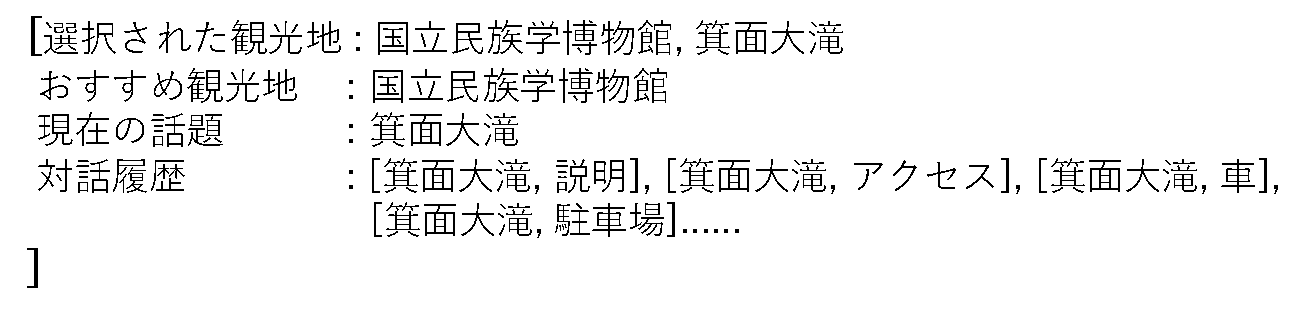
\includegraphics[scale=0.5]{pic/frame.pdf}
    \caption{フレーム表現の例}
    \label{frame}
\end{figure}

私たちは対話の中で主語の省略や指示代名詞をよく使う.例えば,「私は箕面大滝へ行きたいです.そこへはどうやっていきますか.駐車場はありますか.」という文書の場合,「そこ」は直前に述べたを指し,駐車場はありますかという文書には箕面大滝にという語が隠れている.人間はその場の状況を参照し文書の理解を試みるが,システムがなんの情報もなくこの文書を理解することは難しい.このような照応表現の解析は自然言語処理における重要な課題として挙げられ\cite{shouo1996},対話システムの構築においても対話の中での照応解析は大きな問題である\cite{taiwashouo2003}.フレーム表現を利用することで,旅行代理店におけるカウンターセールスという限られた条件の中で,照応解析を実現し,主語の省略や代名詞の使用に対応した人間らしい会話の実現を可能にする.

\subsubsection{行動選択}
内部状態を参照しながら発話理解を行ったのち,行動選択に移る.

\begin{table}[htb]
    \caption{発話行為タイプ}
    \label{sendrecv}
    \centering
    \begin{tabular}{l|l||l|l}
    \hline
    発話行為タイプ     & 説明        & 発話行為タイプ  & 説明\\\hline
    explanation & 概要の説明      & parking  & 駐車場の有無\\
    address     & 住所         & child    & 子供も楽しめるか\\
    time        & 営業時間       & near     & 近隣の飲食店情報\\
    open        & 営業開始時間     & event    & 直近のイベント情報\\
    close       & 営業終了時間     & covid    & covid-19情報\\
    close\_day  & 定休日        & thanks   & お礼\\
    tell        & 電話番号       & yes      & はいと言われた時\\
    accsess     & どうやっていくか   & no       & いいえと言われた時\\
    by\_train   & 電車でのアクセス方法 & stay     & 観光地を迷ってる時 \\
    by\_car     & 車でのアクセス方法  & decision & 観光地を決める時\\
    photo       & 写真撮影の可否    & error    & 対話理解ができなかった時\\
    height      & 観光地の高さ     & benefit  & ご利益(総持寺)\\
    width       & 観光地の広さ    & goshuin  & 御朱印(総持寺)\\
    seasons     & 訪問におすすめの季節 & swim     & 遊泳の可否(箕面大滝)\\ 
    tourists    & 年間観光客数     & choco    & チョコレートの飲食\\
    price       & 発生する料金 & &(明治なるほどファクトリー大阪) \\
\hline
    \end{tabular}   
\end{table}



\subsection{対話を円滑に進める機構}
\subsubsection{対話破綻の抑止}
対話システムがユーザに対して不適切な返答をしてしまう「対話破綻」と呼ばれる現象が起こることがある.対話破綻は大きく4つに分類することができる\cite{challenge2015}.

\begin{enumerate}
    \item 構文などの崩れにより,日本語として成立せず発話そのものが破綻している場合
    \item 日本語としては正しいが,相手の発言に対する「応答」として成立せず破綻している場合
    \item 単発のやりとりとしては成立しているが、既に話した内容と異なる発話をするため,「文脈」が破綻している場合
    \item 社会通念や倫理的におかしな発言をしてしまう場合
\end{enumerate}

体験者の発話から,返答を生成して応答せず,あらかじめ用意された返答を返すため,1つめと4つめの対話破綻は未然に防ぐことができる.また,フレーム表現を用いて対話履歴を参照しながら対話を進めるため,発話の整合性を保ちながら対話を進め,3つめの対話破綻を防ぎながら対話を進める.

2つめの,日本語としては正しいが,相手の発言に対する「応答」として成立せず破綻している場合の典型的な例として,音声認識や発話認識,行動選択をしている間に対話者が新たな発話を行うことで,発話認識,行動選択を再度開始してしまうといったケースが挙げられる.この場合,システムは発話すべきテキストを複数抱えてしまい,円滑に対話が進まなくなる.発話内容とアンドロイドの姿勢・表情の2つの面からこの破綻を防ぐ.

\begin{description}
    \item[発話内容]
    システムが発話を終了する際は全て疑問文で終わる.システムの発言する順番と対話者が発言する順番を明確にすることで,発話認識,行動選択をしている間に対話者が新たな発言をすることを防ぐことができる.
    \item[アンドロイドの姿勢・表情]
    システムが発話を終了した際と音声認識を完了した際に笑顔で頷く.対話者にシステムの発話が終了したことや,音声が正常に認識されたことを表情により示すことで,対話者が不要な発言をすることを防ぐことができる.
\end{description}

\subsubsection{観光地に関する情報の拡充}
6箇所の観光地に関する基本情報として,運営から,るるぶDATA\footnote{旅行ガイドブック「るるぶ情報版」掲載の観光情報コンテンツのデータベース.} \footnote{https://solution.jtbpublishing.co.jp/service/domestic/}を使用した観光案内情報を付与されたが,情報量が不十分であったため,Google Maps APIと手作業による観光地情報の拡充を行なう.

事前にGoogle Maps APIにより観光地周辺の飲食店について情報を収集し,データベースを作成することで,観光地の周辺情報について聞かれた際の返答を用意した.また,「箕面大滝で遊泳することは可能か」,「明治なるほどファクトリーでチョコレートを試食することは可能か」など,各観光地に対して事前に想定される質問への回答を手作業でいくつか用意することで対話の成功確率の向上を試みた.
